\documentclass[cjk,slidestop,compress,mathserif,blue]{beamer}
%dvipdfm选项是关键,否则编译统统通不过
%beamer的颜色选项定义的是导航条和标题的颜色(即关键词structure的颜色)

%%%%%%%%%%%%%%%%仅限于XeTeX可使用的宏包%%%%%%%%%%%%%%%%%%%%%%%%%%%%
\usepackage{fontspec,xunicode,xltxtra,beamerthemesplit}
%\usepackage{beamerthemesplit}
\usepackage{xeCJK}
\setCJKmainfont[BoldFont=黑体, ItalicFont=楷体, BoldItalicFont=仿宋]{黑体}
%\setsansfont[Mapping=tex-text]{Adobe 黑体 Std}
%如果装了Adobe Acrobat,可在font.conf中配置Adobe字体的路径以使用其中文字体
%也可直接使用系统中的中文字体如SimSun,SimHei,微软雅黑 等
%原来beamer用的字体是sans family;注意Mapping的大小写,不能写错

%%%%%%%%   确定标题和导航条结构的框架     %%%%%%%%%%%%
\usepackage{beamerthemeshadow}                       %
%\usepackage{beamerthemeclassic}%导航条色与背景色一致%
%%%%%%%%%%%%%%%%%%%%%%%%%%%%%%%%%%%%%%%%%%%%%%%%%%%%%%
\setbeamerfont{roman title}{size={}}
%\usepackage{CJK} % CJK 中文支持                                  %
\usepackage{amsmath,amsthm,amsfonts,amssymb,bm}
\usepackage{mathrsfs}
\usepackage{xcolor}                                        %使用默认允许使用颜色
\usepackage{enumerate}                                     %使用标注数字
\usepackage{hyperref} 
\usepackage{graphicx}
\usepackage{subfigure}           %图片跨页

%\usepackage[numbers,sort&compress]{natbib} %紧密排列             %
\usepackage[sectionbib]{chapterbib}        %每章节单独参考文献   %
\usepackage{hypernat}                                                                         %
%\usepackage[dvipdfm,bookmarksopen=true,pdfstartview=FitH,CJKbookmarks]{hyperref}		%
\hypersetup{bookmarksnumbered,colorlinks,linkcolor=brown,citecolor=blue,urlcolor=red}         %
%参考文献含有超链接引用时需要下列宏包,注意与natbib有冲突        %
%\usepackage[dvipdfm]{hyperref}                                  %
%\usepackage{hypernat}                                           %
\newcommand{\upcite}[1]{\hspace{0ex}\textsuperscript{\cite{#1}}} %

%\useoutertheme{smoothbars}
\useinnertheme[shadow=true]{rounded}
\usetheme{Berkeley}                                          %主题式样
%\usetheme{Luebeck}

\usecolortheme{lily}                                        %颜色主题式样

\usefonttheme{professionalfonts}                           %字体主题样式宏包

%\beamertemplatetransparentcoveredhigh                      %使所有被隐藏的文本高度透明
\beamertemplatetransparentcovereddynamicmedium             %使所有被隐藏的文本完全透明,动态,动态的范围很小
\mode<presentation>
%\beamersetaveragebackground{gray}                          %设置背景颜色(单一色) 
\beamertemplateshadingbackground{green!10}{red!5}         %设置背景颜色(渐变色)

%i放置单位logo
%\logo{
\includegraphics[width=1.6cm,height=0.35cm]{Figures/BCC_logo-1.png}}	%简单设置logo

%\pgfdeclareimage[width=3.5cm]{logoname}{Figures/BCC_logo-1.png}		%logo置于左侧微调
%\logo{\pgfuseimage{logoname}{\vspace{0.2cm}\hspace*{-2.0cm}}}

%在指定位置精确放置logo
\usepackage{tikz}
\usepackage{beamerfoils}
\usepackage{pgf}
\logo{\pgfputat{\pgfxy(11.68,0.15)}{
\includegraphics[height=1.01cm,viewport=0 0 140 120,clip]{Figures/BCC_logo-1.png}}\pgfputat{\pgfxy(10.502,-0.218)}{
\includegraphics[height=0.369cm,viewport=140 0 540 120,clip]{Figures/BCC_logo-1.png}}}
%\logo{\pgfputat{\pgfxy(11.68,0.15)}{
\includegraphics[height=0.95cm,viewport=0 0 510 360,clip]{Figures/Logo_Gainstrong.png}}\pgfputat{\pgfxy(10.333,-0.195)}{
\includegraphics[height=0.35cm,viewport=530 70 1100 218,clip]{Figures/Logo_Gainstrong.png}}}
%\MyLogo{
%	\pgfputat{\pgfxy(-50,-50)}{\pgfbox[right,base]{
\includegraphics[height=1cm]{Figures/BCC_logo-1.png}}}

%logo作为背景放置
%\setbeamertemplate{background}{
%	\pgfputat{\pgfxy(6.5,-0.5)}{\pgfbox[left,top]{\pgfimage[height=1.1cm]{Figures/BCC_logo-1.png}}}}

%\logo{}									%不显示logo

\begin{document}
%\begin{CJK*}{GBK}{song}
%\begin{CJK*}{GBK}{kai}
%beamer下不能用\songyi、\zihao等命令!
%\graphicspath{Figures/}

%-------------------------------PPT Title-------------------------------------
\title{光学函数的计算}
%-----------------------------------------------------------------------------

%----------------------------Author & Date------------------------------------
\author{北京市计算中心\;云平台\:姜骏}
\date{\textrm{2017.01.04}}
%\date{2013.09.10}
\frame{\titlepage}
%-----------------------------------------------------------------------------

%------------------------------------------------------------------------------列出全文 outline ---------------------------------------------------------------------------------
\section*{}
\frame[allowframebreaks]
{
  \frametitle{Outline}
%  \frametitle{\textcolor{mycolor}{\secname}}
  \tableofcontents%[current,currentsection,currentsubsection]
}
%在每个section之前列出全部Outline
%类似的在每个subsection之前列出全部Outline是\AtBeginSubsection[]
\AtBeginSection[]
{
  \frame<handout:0>
  {
    \frametitle{Outline}
%全部Outline中,本部分加亮
    \tableofcontents[current,currentsection]
  }
}

%------------------------------------------------------------------------------PPT main Body------------------------------------------------------------------------------------
\small
\section{光学常数间的基本关系}
\frame
{
	\frametitle{固体光学常数间的基本关系}
	光(电磁波)通过固体材料时,电磁波将与固体中的电子、原子(离子)间相互作用,因此发生光吸收
	\begin{itemize}
		\item 角频率为$\omega$的电磁波(横波)在均匀介质中传播(设定为$x$方向)
			\begin{displaymath}
				\mathbf{E}(\vec r,t)=E(z)\mathrm{e}^{-\mathrm{i}\omega t}(1,0,0)\qquad\mathbf{E}\parallel x
			\end{displaymath}
			根据\textrm{Maxwell~}方程,可有电场与电流密度的基本关系
			\begin{displaymath}
				\frac{\mathrm{d}^2E(z)}{\mathrm{d}z^2}=-\frac{\omega^2}{c^2}E(z)-\frac{4\pi\mathrm{i}\omega}{c^2}J(z)
			\end{displaymath}
		\item 引入复数电导率$\sigma(\sigma)=\sigma_1(\omega)+\mathrm{i}\sigma_2(\omega)$
			\begin{displaymath}
				J(z)=\sigma(\omega)E(z)=\sigma_1(\omega)E(z)+\mathrm{i}\sigma_2(\omega)E(z)
			\end{displaymath}
			吸收介质中电流$\mathbf{j}$分为两部分,一部分与$\mathbf{E}$相位差$90^{\circ}$,称为\textcolor{magenta}{极化电流},一部分与电场$\mathbf{E}$同相位,称为\textcolor{magenta}{传导电流}\\
			\textcolor{red}{注意}:~极化电流与电场相位差$90^{\circ}$,在一个周期平均电场做工为零,不消耗电磁场能量
	\end{itemize}
}

\frame
{
	\frametitle{固体光学常数间的基本关系}
	\begin{itemize}
		\item 当载流子迁移距离比电磁波的波长小得多时(长波极限),可忽略电磁波在空间变化的影响
			\begin{displaymath}
				\frac{\mathrm{d}^2E(z)}{\mathrm{d}z^2}=-\frac{\omega^2}{c^2}\left[ 1+\frac{4\pi\mathrm{i}\omega\sigma(\omega)}{\omega} \right]E(z)
			\end{displaymath}
		可解得电磁波在介质内的衰减
		\begin{displaymath}
			E(z)=E_0\mathrm{e}^{\mathrm{i}(\omega/c)Nz}
		\end{displaymath}
		这里$N$是复数折射率,满足
		\begin{displaymath}
			N^2=1+\frac{4\pi\mathrm{i}\sigma(\omega)}{\omega} 
		\end{displaymath}
		\item 复数折射写成$N=n+\mathrm{i}k$,其中$n$是折射指数,$k$是消光系数,因此
			\begin{displaymath}
				E(z)=E_0\mathrm{e}^{\mathrm{i}(\omega/c)nz}\mathrm{e}^{-(\omega/c)kz}
			\end{displaymath}
			因此电磁波在介质中传播速度$c/n$,透射深度$\delta(\omega)=\frac{c}{\omega k(\omega)}$
	\end{itemize}
}

\frame
{
	\frametitle{固体光学常数间的基本关系}
	\begin{itemize}
		\item 吸收系数
			\begin{displaymath}
				\alpha(\omega)=\frac{2\omega k(\omega)}c\equiv\frac2{\delta(\omega)}
			\end{displaymath}
		\item 电磁波在介质中传播,根据介电函数和复数折射率的关系$N^2=\varepsilon$,因此
			\begin{displaymath}
				\varepsilon_1=n^2-k^2\qquad\varepsilon_2=2nk
			\end{displaymath}
			相应地
			\begin{displaymath}
				n^2=\frac12(\varepsilon_1+\sqrt{\varepsilon_1^2+\varepsilon_2^2})\quad k^2=\frac12(-\varepsilon_1+\sqrt{\varepsilon_1^2+\varepsilon_2^2})
			\end{displaymath}
			根据等式$\varepsilon(\omega)=1+\dfrac{4\pi\mathrm{i}\sigma(\omega)}{\omega}$有
			\begin{displaymath}
				\varepsilon_1=1-\frac{4\pi\sigma_2(\omega)}{\omega}\qquad\varepsilon_2=\frac{4\pi\sigma_1(\omega)}{\omega} 
			\end{displaymath}
			\textcolor{red}{注意}:~\textcolor{blue}{确定介电函数虚部与电导率实部间的关系}
	\end{itemize}
}

\frame
{
	\frametitle{固体光学常数间的基本关系}
	\begin{itemize}
		\item 电磁波垂直入射时,反射波与入射波分别为
\begin{figure}[h!]
\centering
%\hspace*{-10pt}
\vspace*{-0.4in}
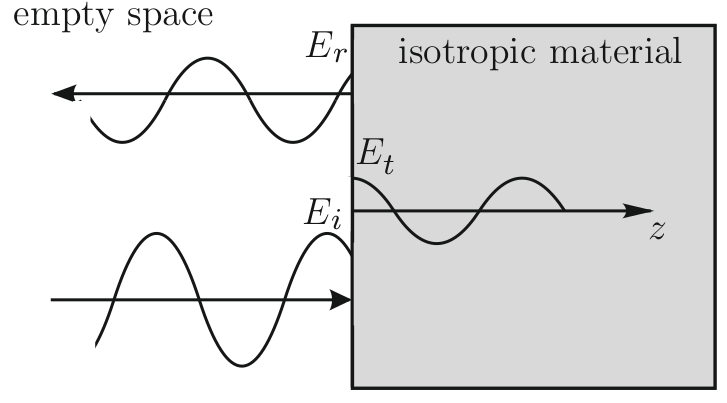
\includegraphics[height=1.2in,width=1.8in,viewport=0 0 750 600,clip]{Figures/Optic-reflect.png}
\caption{\small \textrm{Schematic representation of incident, reflected and transmitted electromagnetic wave at the surface.}}%
\label{Optic-reflect}
\end{figure} 
			\begin{displaymath}
				\begin{aligned}
					&E(z)=E_t\mathrm{e}^{\mathrm{i}(\omega/c)Nz}\quad z>0\\
					&E(z)=E_i\mathrm{e}^{\mathrm{i}(\omega/c)z}+E_r\mathrm{e}^{-\mathrm{i}(\omega/c)z}\quad z<0\\
				\end{aligned}
			\end{displaymath}
			反射率$R$可以表示为
			\begin{displaymath}
				R=\left|\frac{E_r}{E_i}\right|^2=\left|\frac{1-N}{1+N}\right|^2=\frac{(n-1)^2+k^2}{(n+1)^2+k^2}
			\end{displaymath}
	\end{itemize}
}

\section{自由载流子与\rm{Drude}模型}
\frame
{
	\frametitle{自由电子的\textrm{Drude}模型}
	\textcolor{blue}{在远红外区,经典自由电子气模型可以很好地描述金属的光学行为}
	\begin{itemize}
		\item 载流子在外电场$\mathbf{E}(\vec r,t)=\mathbf{E}_0\mathrm{e}^{\mathrm{i}(\vec q\cdot\vec r-\omega t)}$下的运动方程
			\begin{displaymath}
				m\ddot{\vec r}=-\frac m{\tau}\dot{\vec r}+(-e)\mathbf{E}_0\mathrm{e}^{\mathrm{i}(\vec q\cdot\vec r-\omega t)}
			\end{displaymath}
			这里$\vec r(t)$是载流子坐标,$\tau$是\textcolor{red}{唯象弛豫时间}
		\item 长波极限下,忽略电磁波在空间的变化
			\begin{displaymath}
				m\ddot{\vec r}=-\frac m{\tau}\dot{\vec r}-e\mathbf{E}_0\mathrm{e}^{\mathrm{i}-\omega t}
			\end{displaymath}
			取载流子位置函数$\vec r(t)=\vec A_0\mathrm{e}^{-\mathrm{i}\omega t}$,有
			\begin{displaymath}
				\vec A_0=\frac{e\tau}m\frac1{\omega(\mathrm{i}+\omega\tau)}\mathbf{E}_0
			\end{displaymath}
	\end{itemize}
}

\frame
{
	\frametitle{自由电子的\textrm{Drude}模型}
	如果载流子密度为$n$,则电流密度
	\begin{displaymath}
		\mathbf{J}=n(-e)\dot{\vec r}=n(-e)(-\mathrm{i}\omega)\vec A_0\mathrm{e}^{-\mathrm{i}\omega t}=\frac{ne^2\tau}m\frac1{1-\mathrm{i}\omega\tau}\mathbf{E}_0\mathrm{e}^{-\mathrm{i}\omega t}
	\end{displaymath}
	由此可得频率有关的电导率表示为
	\begin{displaymath}
		\sigma(\omega)=\frac{ne^2\tau}m\frac1{1-\mathrm{i}\omega\tau}=\sigma_0\frac1{1-\mathrm{i}\omega\tau}
	\end{displaymath}
	其中$\sigma_0=ne^2\tau/m$是静态电导率
	\begin{itemize}
		\item 介电函数可表示为
			\begin{displaymath}
				\varepsilon(\omega)=1-\frac{\omega_\mathrm{p}^2}{\omega(\omega+\mathrm{i}/\tau)}=\underline{\textcolor{blue}{\left[ 1-\frac{\omega_{\mathrm{p}}^2\tau^2}{1+\omega^2\tau^2} \right]}}+\mathrm{i}\underline{\textcolor{blue}{\left[ \frac{\omega_{\mathrm{p}}^2\tau}{\omega(1+\omega^2\tau^2)} \right]}}
			\end{displaymath}
			其中$\omega_{\mathrm{p}}$是载流子的等离振荡频率
			\begin{displaymath}
				\omega_{\mathrm{p}}^2=\frac{4\pi ne^2}m
			\end{displaymath}
%\begin{displaymath}
%	\epsilon_1(\omega)=1-\frac{\omega_{\mathrm{p}}^2\tau^2}{1+\omega^2\tau^2}\quad \epsilon_2(\omega)=\frac{\omega_{\mathrm{p}}^2\tau}{\omega(1+\omega^2\tau^2)}\quad
%\end{displaymath}
	\end{itemize}
}

\section{固体的光吸收过程}
\frame
{
\frametitle{带间跃迁的计算}
\begin{itemize}
\setlength{\itemsep}{10pt}
	\item 用半经典方法处理周期性体系的光学性质,用量子力学处理介质,对电磁波仍然采用经典电动力学描写
	\item 以半导体中的带间垂直跃迁(价带$|v,\vec k\rangle$,导带$|c,\vec k\rangle$)为例讨论固体的能带间跃迁
\begin{figure}[h!]
\centering
%\hspace*{-10pt}
\vspace*{-0.3in}
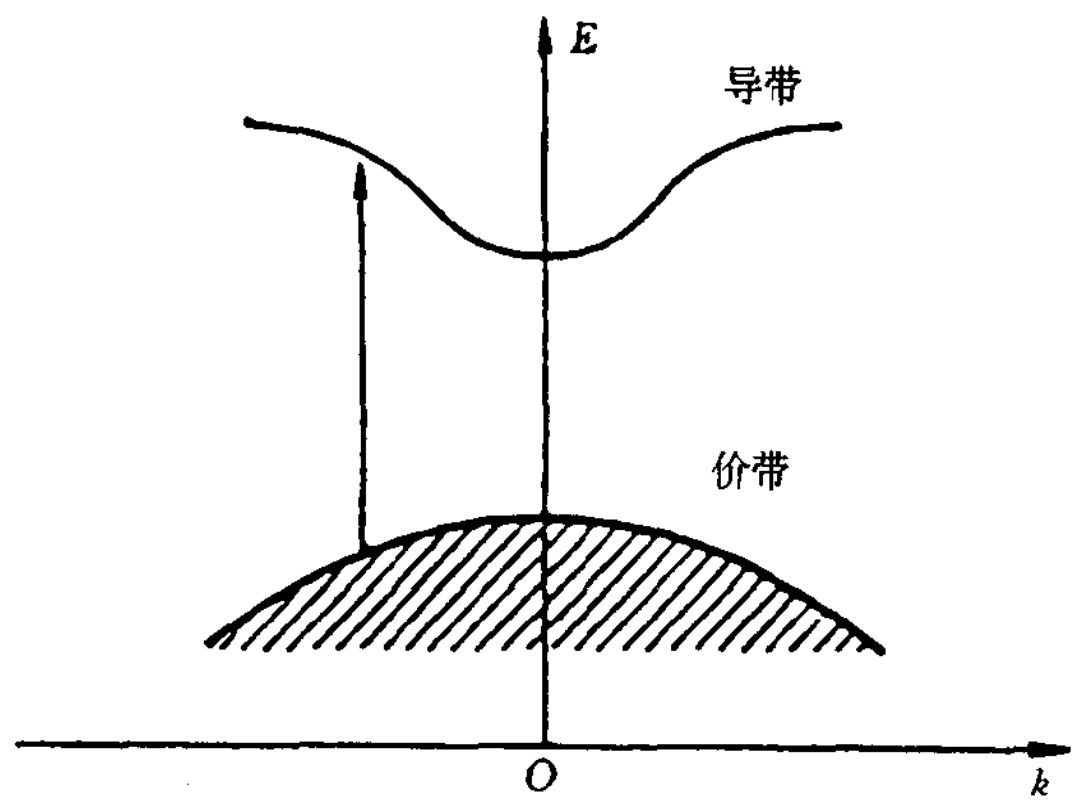
\includegraphics[height=1.8in,width=2.0in,viewport=0 0 1000 900,clip]{Figures/optic_dir.png}
\caption{\small \textrm{Schematic representation of directly inter-band transition.}}%
\label{Optic-dir}
\end{figure} 
\end{itemize}
}

\frame
{
	\frametitle{带间跃迁的计算}
\begin{itemize}
晶体中动量为$\vec p$的电子在电磁场(电磁场矢量势为$\vec A$)存在情况下,应用含时微扰理论,
\begin{displaymath}
	\hspace*{-20pt}
	H=\frac1{2m}[\vec p+\frac{e}c\mathbf{A}(\vec r,t)]^2+V(\vec r)=\left[ \frac{\vec p^2}{2m}+V(\vec r) \right]+\frac{e}{mc}\mathbf{A}\cdot\vec p+\frac{e^2}{2mc^2}\mathbf{A}^2
\end{displaymath}
其中电磁波
\begin{displaymath}
	\mathbf{A}(\vec r,t)=A_0\mathbf{e}\mathrm{e}^{\mathrm{i}(\vec q\cdot\vec r-\omega t)}+\mathrm{c.c}\quad\mathbf{e}\bot\vec q
\end{displaymath}
准确到$\vec A$的线性项(忽略$\vec A$的平方项)\textrm{Hamiltonian}为:
\begin{displaymath}
	H=\left[ \frac{\vec p^2}{2m}+V(\vec r) \right]+\frac{eA_0}{mc}\mathrm{e}^{\mathrm{i}(\vec q\cdot\vec r-\omega t)}\mathbf{e}\cdot\vec p+\frac{eA_0}{mc}\mathrm{e}^{-\mathrm{i}(\vec q\cdot\vec r-\omega t)}\mathbf{e}\cdot\vec p
\end{displaymath}
	\item 频率为$\omega$的平面偏振光,电场和磁场的强度为
\begin{displaymath}
%  \left\{
\begin{aligned}
    \vec E&=-\frac1c\frac{\partial\vec A}{\partial t}\\
    \vec B&=\nabla\times\vec A
  \end{aligned}%\right.
  \label{eq:optic-26}
\end{displaymath}
\end{itemize}
%式中$c$为光速。
}

\frame
{
\frametitle{带间跃迁的计算}
在含时微扰\textrm{Hamiltonian}作用下,带间垂直跃迁为
\begin{displaymath}
	\begin{aligned}
		W(\vec q,\omega)=&\frac{2\pi}{\hbar}\left( \frac{eA_0}{m_ec} \right)^22\sum_{i,j}|\langle c,\vec k|\mathrm{e}^{\mathrm{i}\vec q\cdot\vec r}\mathbf{e}\cdot\vec p|v,\vec k\rangle|^2\\
		\times&\delta[E_c(\vec k)-E_v(\vec k)-\omega][f(E_c(\vec k))-f(E_v(\vec k))]
	\end{aligned}
  \label{eq:optic-27}
\end{displaymath}
$\delta$因子表示跃迁过程的能量守恒关系%,矩阵元$\langle c\vec k|H'|v\vec k\rangle$表示\textrm{Bloch}函数间的积分
。对垂直跃迁,忽略磁场贡献,%矩阵元可以简写成$\dfrac1cA_0\vec e\cdot\vec M_{cv}(\vec k)$,$\vec s$为电磁波矢量势$\vec A_0(=A_0\vec s)$方向的单位矢量。
只有满足能量守恒和动量守恒条件的跃迁才对积分有贡献。%$\displaystyle\int W\dfrac{\textrm{d}\vec k}{(2\pi)^3}$为单位体积、单位时间内吸收能量为$\omega$的光子的总数,系数2是考虑两种自旋态。将式\eqref{eq:optic-27},\eqref{eq:optic-28}代入式\eqref{eq:optic-29},并应用$\dfrac{A_0}c\vec e\cdot\vec M_{cv}(\vec k)$表示矩阵元,得

电磁波在介质中产生的电场
\begin{displaymath}
	\mathbf{E}(\vec r,t)=-\frac1c\frac{\partial\mathbf{A}}{\partial t}=E_0\mathbf{e}\mathrm{e}^{\mathrm{i}\vec q\cdot\vec r-\omega t}+\mathrm{c.c}\quad\mbox{其中}E_0=\mathrm{i}\omega\frac{A_0}c
\end{displaymath}

介质中的传导电流
\begin{displaymath}
	\mathbf{J}(\vec r,t)=\sigma(\vec q,\omega)E_0\mathbf{e}\mathrm{e}^{\mathrm{i}(\vec q\cdot\vec r-\omega t)}+\mathrm{c.c}\quad(\mathbf{e}\bot\vec q)
\end{displaymath}
由此计算得到吸收功率
\begin{displaymath}
	\int_V\mathbf{J}\cdot\mathbf{E}\mathrm{d}\vec r=2\sigma_1(\vec q,\omega)|E_0|^2V=2\sigma_1(\vec q,\omega)\frac1{c^2}\omega^2A_0^2V=\textcolor{blue}{\hbar\omega W(\vec q,\omega)}
\end{displaymath}
}

\frame
{
	\frametitle{带间跃迁的计算}
长波极限下($\vec q\rightarrow0$), 根据光学性质的基本关系,可有介电函数的介电函数虚部表达式
\begin{displaymath}
	\begin{aligned}
		\varepsilon_2(\omega)=&\lim_{\vec q\rightarrow0}\frac{8\pi^2e^2}{m_e^2\omega^2}\int\frac{\mathrm{d}\vec k}{(2\pi)^3}|\langle c,\vec k|\mathbf{e}\cdot\vec p|v,\vec k\rangle|^2\\
		\times&\delta(E_c(\vec k)-E_v(\vec k)-\hbar\omega)[f(E_c(\vec k))-f(E_v(\vec k))]
	\end{aligned}
  \label{eq:optic-varepsilon_2}
\end{displaymath}
$\varepsilon_2(\omega)$是晶体的光学吸收和能带结构之间的基本关系

对应的$\varepsilon_1$可以根据\textrm{Kramers-Kr\"onig}关系%\eqref{eq:optic-16}
得到
\begin{displaymath}
	\varepsilon_1(\omega)=1+\frac1{\pi}\mathscr{P}\int_{-\infty}^{+\infty}\frac{\varepsilon_2(\omega^{\prime})}{\omega^{\prime}-\omega}\textrm{d}\omega^{\prime}=1+\frac2{\pi}\mathscr{P}\int_0^{+\infty}\frac{\omega^{\prime}\varepsilon_2(\omega^{\prime})}{\omega^{\prime2}-\omega^2}\textrm{d}\omega^{\prime}
  \label{eq:optic-varepsilon_1}
\end{displaymath}
因此介电函数表示为
\begin{displaymath}
	\hspace*{-10pt}
	\varepsilon(\omega)=1+\frac{8\pi e^2}{m_e^2}\int\frac{\mathrm{d}\vec k}{(2\pi)^3}\frac{|\langle c,\vec k|\mathbf{e}\cdot\vec p|v,\vec k\rangle|^2}{(E_c(\vec k)-E_v(\vec k))/\hbar^2}\frac{(-\mathrm{i})[f(E_c(\vec k))-f(E_v(\vec k))]}{E_c(\vec k)-E_v(\vec k)-\hbar\omega-\mathrm{i}\eta}
  \label{eq:optic-varepsilon}
\end{displaymath}
}

\frame
{
	\frametitle{带间跃迁和带内跃迁的计算}
电导率函数可表示为
\begin{displaymath}
	\sigma(\omega)=\frac{2e^2}{m_e^2}\int\frac{\mathrm{d}\vec k}{(2\pi)^3}\frac{|\langle c,\vec k|\mathbf{e}\cdot\vec p|v,\vec k\rangle|^2}{(E_c(\vec k)-E_v(\vec k))/\hbar}\frac{(-\mathrm{i})[f(E_c(\vec k))-f(E_v(\vec k))]}{E_c(\vec k)-E_v(\vec k)-\hbar\omega-\mathrm{i}\eta}
  \label{eq:optic-sigma}
\end{displaymath}

\textcolor{violet}{推广到长波极限下的带内跃迁}
\begin{displaymath}
	f(E_c(\vec k))-f(E_v(\vec k))\approx\frac{\partial f}{\partial E}(f(E_c(\vec k))-f(E_v(\vec k)))
\end{displaymath}
\begin{displaymath}
	\sigma(\omega)=\frac{e^2\hbar}{4\pi^3}\int\mathrm{d}\vec k\langle c,\vec k|\mathbf{e}\cdot\vec p|v,\vec k\rangle|^2\frac{-\mathrm{i}}{E_c(\vec k)-E_v(\vec k)-\hbar\omega-\mathrm{i}\eta}\left( -\frac{\partial f}{\partial E} \right)
\end{displaymath}
引入等式$\eta=\hbar/\tau$,并作展开
\begin{displaymath}
	E_{\vec k+\vec q}-E_{\vec k}\approx\vec q\cdot(\partial E/\partial\vec k)=\frac{\hbar}{m_e}\langle c,\vec k|\mathbf{q}\cdot\vec p|v,\vec k\rangle
\end{displaymath}
由此可得
\vspace{-5pt}
\begin{displaymath}
	\sigma(\vec q,\omega)=\frac{e^2}{4\pi^3}\int\mathrm{d}\vec k\frac{\tau|\langle c,\vec k|\mathbf{e}\cdot\vec p|v,\vec k\rangle|^2}{1-\mathrm{i}\tau(\omega-\langle c,\vec k|\mathbf{q}\cdot\vec p|v,\vec k\rangle)}\left( -\frac{\partial f}{\partial E} \right)
\end{displaymath}
}

\frame
{
\frametitle{联合态密度(Joint DOS, JDOS)}
定义联合态密度(\textrm{Joint Density of States, JDOS})
\begin{displaymath}
  J_{cv}(\hbar\omega)=\sum_{v,c}\int\delta[E_c(\vec k)-E_v(\vec k)-\omega]\frac{2\textrm{d}\vec k}{(2\pi)^3}
  \label{eq:optic-33}
\end{displaymath}
令$E_{cv}(\vec k)$\,=\,$E_c(\vec k)-E_v(\vec k)$,因$\textrm{d}\vec k$\,=\,$\dfrac{dE_{cv}(\vec k)}{\nabla_{\vec k}E_{cv}(\vec k)}\textrm{d}S$,故有
\begin{displaymath}
  J_{cv}(\omega)=\frac2{(2\pi)^3}\sum_{v,c}\int\limits_{E_{cv}(\vec k)=\omega}\frac{\textrm{d}S}{\nabla_{\vec k}E_{cv}(\vec k)}
  \label{eq:optic-34}
\end{displaymath}
类似态密度的定义,而$E_{cv}(\vec k)$同时联系着价带和导带,因此称为联合态密度。当矩阵元$\vec M_{cv}(\vec k)$随波矢$\vec k$变化比较小的时候,可以近似地认为$\varepsilon_2(\omega)\!\propto\!J_{cv}(\omega)$。满足$|\nabla_{\vec k}E_{cv}(\vec k)|\!=\!0$的$\vec k$点,是联合态密度$J_{cv}(\omega)$和$\varepsilon_2(\omega)$的奇点(\textrm{Van Hove}奇点或临界点),在这些点,$J_{cv}(\omega)$和$\varepsilon_2(\omega)$%的能谱图将出现典型结构(即
对能量的微商呈现典型的不连续。%联合态密度的奇点有两种情况,即$\nabla_{\vec k}E_c(\vec k)\!=\!\nabla_{\vec k}E_v(\vec k)\!=\!0$和$\nabla_{\vec k}E_c(\vec k)\!=\!\nabla_{\vec k}E_v(\vec k)\!\neq\!0$。将$E_{cv}(\vec k)$在奇点作Taylor级数展开到二级,$$E_{cv}(\vec k)=E_0+a_xk_x^2+a_yk_y^2+a_zk_z^2$$可以看出有四种类型的奇点:
}

\section{磁光\rm{Kerr~}效应}
\frame
{
	\frametitle{磁光\textrm{Kerr~}效应}
	\begin{itemize}
		\item 外磁场存在时,晶体沿外磁场方向表现处轴各向异性。磁光\textrm{Kerr~}效应是表征晶体在磁场存在时表现出的光学轴各向异性
		\item 磁光\textrm{Kerr~}效应和\textrm{Hall~}效应的微观机理类似,\textrm{Hall~}效应可以视为磁光\textrm{Kerr~}效应的静态极限
		\item \textcolor{blue}{\textrm{Kerr~}效应}:~入射平面偏振光可分解为两个圆偏振光,介质对两个圆偏振光吸收不同,导致出射光的偏振态发生转变\\\textrm{Kerr~}效应可用偏转角$\theta_K$和椭圆率$\varepsilon_K$表征
\begin{figure}[h!]
\centering
%\hspace*{-10pt}
\vspace*{-0.4in}
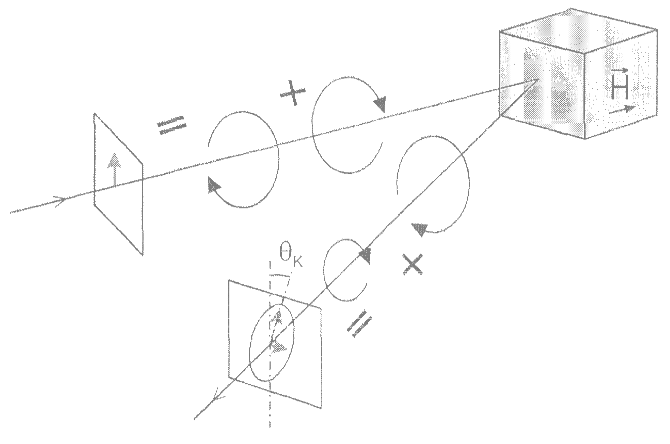
\includegraphics[height=1.5in,width=2.0in,viewport=0 0 750 550,clip]{Figures/Magopt_Kerr.png}
\caption{\small \textrm{Schematic representation of Kerr effect.}}%
\label{Optic-Kerr}
\end{figure} 
	\end{itemize}
}

\frame
{
	\frametitle{磁光\textrm{Kerr~}效应}
	取外加磁场方向为$z$轴正方向,垂直入射的平面偏振光波矢$\vec q$平行于外磁场($\vec q\parallel\vec H$),在折射率为$N$的介质表面被反射,入射光沿$-z$方向传播,电矢量
	\begin{displaymath}
		\mathbf{E}_{\pm}(z,t)=E_0\mathrm{e}^{\mathrm{i}(2\pi N_{\pm}z/\lambda_0-\omega t)}(\mathbf{e}_x\pm\mathrm{i}\mathbf{e}_y)
	\end{displaymath}
	这里符号$+$和$-$分别标记\textcolor{blue}{右圆偏振光}(\textrm{right circular polarisation, RCP})和\textcolor{blue}{左圆偏振光}(\textrm{left circular polarisation, LCP})\\
	$\lambda_0$是入射偏振光的真空波长\\
	$N_{\pm}$是介质对两种不同偏振光的复数折射系数\\
	$\mathbf{e}_x$和$\mathbf{e}_y$是$x-$和$y-$方向的电场单位矢量
	\begin{displaymath}
		\begin{aligned}
			\theta_K=&-\frac12(\theta_+-\theta_-)\\
			\varepsilon_K=&\arctan\left( -\frac{|r|_+-|r|_-}{|r|_++|r|_-} \right)
		\end{aligned}
	\end{displaymath}
}

\frame
{
	\frametitle{磁光\textrm{Kerr~}效应}
	偏转角与偏振光的复数折射关系
	\begin{displaymath}
		\begin{aligned}
			&\theta_{\pm}=\arctan\left( -\frac{2k_{\pm}}{n_{\pm}^2+k_{\pm}^2-1} \right)\\
			&|r|_{\pm}=\frac{\sqrt{(n_{\pm}^2+k_{\pm}^2-1)^2+(2k_{\pm})^2}}{(n_{\pm}+1)^2+k_{\pm}^2}
		\end{aligned}
	\end{displaymath}
	各向异性材料的复数光学函数$\varepsilon$和$\sigma$是\textcolor{red}{二阶张量}:\\
	当外加磁场$\mathbf{H}$(取磁场方向为$z$方向,$\mathbf{H}=H_z$),张量不再对角化,非对角元出现在垂直于磁场的平面(即$xy-$面)内
	\begin{displaymath}
		\tilde\sigma=\left(
		\begin{matrix}
			\sigma_{xx} &\sigma_{xy} &0\\
			-\sigma_{xy} &\sigma_{xx} &0\\
			0 &0 \sigma_{zz}
		\end{matrix}\right)
	\end{displaymath}
	这里$\sigma_{lj}=\sigma_1^{lj}+\mathrm{i}\sigma_2^{lj}$
}

\frame
{
	\frametitle{磁光\textrm{Kerr~}效应}
	二阶张量矩阵元与圆偏振光电导率满足
	\begin{displaymath}
		\sigma_{\pm}=\sigma_{xx}\pm\mathrm{i}\sigma_{xy}
	\end{displaymath}
	因此
	\begin{displaymath}
		\begin{aligned}
			&\sigma_{xx}=(\sigma_++\sigma_-)/2\\
			&\sigma_{xy}=(\sigma_+-\sigma_-)/2\mathrm{i}
		\end{aligned}
	\end{displaymath}
	对于小角度\textrm{Kerr~}偏转($\theta_K\leqslant10^{\circ}\sim12^{\circ}$),近似有
	\begin{displaymath}
		\begin{aligned}
		\sin(\theta_+-\theta_-)&\approx\theta_+-\theta_-\qquad \cos(\theta_+-\theta_-)\approx1\\
		&(|r|_+-|r|_-)^2\ll2|r|_+|r|_-
		\end{aligned}
	\end{displaymath}
	可以证明
	\hspace{-50pt}
	\begin{displaymath}
		\begin{aligned}
			&\mbox{\textcolor{blue}{\rm{Kerr~}效应}:~}\quad&\Phi_K=\theta_K(\omega)+\mathrm{i}\varepsilon_K(\omega)\approx\frac{-\sigma_{xy}}{\sigma_{xx}\sqrt{1+\frac{4\pi\mathrm{i}}{\omega}\sigma_{xx}}}\\
			&\mbox{\textcolor{blue}{\rm{Faraday~}效应}:~}\quad&\Phi_F=\theta_F(\omega)+\mathrm{i}\varepsilon_F(\omega)\approx\frac{\sigma_{xy}}{\sqrt{1+\frac{4\pi\mathrm{i}}{\omega}\sigma_{xx}}}\frac{2\pi}c
		\end{aligned}
	\end{displaymath}
}

\section{非线性光学}
\frame
{
	\frametitle{非线性光学}
	材料对强激光束的响应,一般需要考虑\textcolor{purple}{非线性效应}
\begin{itemize}
	\item 非线性光学主要应用于光谱学、电信和天文学等的基础研究
	\item \textcolor{blue}{倍频效应}(\textrm{SHG})主要用于磁性材料的表面结构研究
\begin{figure}[h!]
\centering
\vspace*{-0.2in}
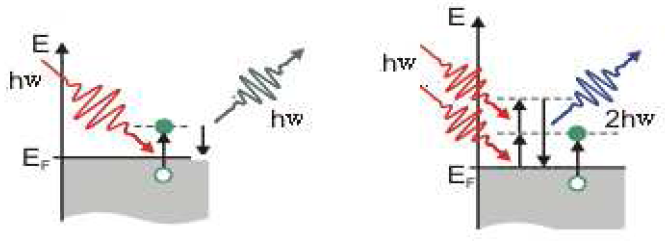
\includegraphics[height=0.9in,width=2.0in,viewport=0 0 700 250,clip]{Figures/nlo-optic.png}
\caption{\small \textrm{Schematic representation of linear optical transition and second harmonic generation (SHG).}}%
\label{nlo-optic}
\end{figure} 
\end{itemize}
\vspace{-12pt}
\begin{displaymath}
	\mathbf{P}^{\alpha}(\omega)=\chi_{ab}^{(1)}\cdot\mathbf{E}^b(\omega)+\chi_{abc}^{(2)}\cdot\mathbf{E}^b(\omega)\cdot\mathbf{E}^c(\omega)+\cdots
\end{displaymath}
{\fontsize{8.5pt}{8pt}\selectfont{这里$\chi^{(1)}$是线性光学极化率(两阶张量),$\chi^{(2)}$是二阶光学极化率(三阶张量)}}\\
倍频效应的光学极化率一般记作$\chi^{(2)}(2\omega,\omega,\omega)$
%\vspace{5pt}
%关于非线性光学极化率,具体可参阅文献\cite{arXiv-0305016v2,PRB71-125107_2005}及相关文献
}

\frame
{
	\frametitle{非线性光学:~\textrm{SHG}的$\chi^{(2)}(2\omega,\omega,\omega)$的计算}
	为计算光学性质,在独立粒子近似下,考虑交变电场后的\textrm{Hamiltonian}
	\begin{displaymath}
		H(t)=\sum_i\frac{(\vec p_i-\mathbf{K}(t))^2}2+V(\vec x_i)
	\end{displaymath}
	这里$i$标记位于坐标$\vec x_i$的电子\\
	$\vec p$是动量算符$\vec p_i=-\mathrm{i}\nabla_i$\\
	$V(\vec x)$是有效周期势\\
	当外加交变电磁场为$\mathbf{A}(t)$,$\mathbf{K}(t)=\mathbf{A}/c$,因此交变电场$\mathbf{E}(t)=-\dot{\mathbf{A}}(t)/c$\\
	\textcolor{violet}{长波极限下},$H(t)$分解成时间无关部分$H_0$和时间相关部分
	\begin{displaymath}
		H(t)=H_0+H_1(t)+H_2(t)
	\end{displaymath}
	其中\vspace{-12pt}
	\begin{displaymath}
		\begin{aligned}
			&H_0=\sum_iH_{0i}=\frac12\sum_i\vec p_i^2+V(\vec x_i)\\
			&H_1(t)=-\mathbf{K}(t)\sum_i\vec p_i\qquad H_2(t)=\frac12N\mathbf{K}^2(t)
		\end{aligned}
	\end{displaymath}
}

\frame
{
	\frametitle{非线性光学:~\textrm{SHG}的$\chi^{(2)}(2\omega,\omega,\omega)$的计算}
	\textcolor{red}{长波极限下,$H_2$只是对波函数引入相因子,因此可忽略;~将$H_1$视为微扰}
	\begin{displaymath}
		\begin{aligned}
			H_0\psi_n(\vec k,\vec x)=&\omega_n(\vec k)\psi_n(\vec k,\vec x)\\
			\psi_n(\vec k,\vec x)=&\Omega^{-1/2}u_n(\vec k,\vec x)\mathrm{e}^{\mathrm{i}\vec k\cdot\vec x}
		\end{aligned}
	\end{displaymath}
	考虑上述时间相关\textrm{Hamiltonian}后
	\begin{displaymath}
		\bar\psi_n(\vec k,\vec x)=\Omega^{-1/2}u_n(\vec k+\mathbf{K}(t),\vec x)\mathrm{e}^{\mathrm{i}\vec k\cdot\vec x}
	\end{displaymath}
	满足
	\begin{displaymath}
		H(t)\bar\psi_n(\vec k,\vec x)=\omega_n(\vec k+\mathbf{K}(t))\bar\psi_n(\vec k,\vec x)
	\end{displaymath}
	选择正交的基$\bar\psi_n(\vec k,\vec x)$,通过$\mathbf{K}(t)$与时间$t$相关,
	\begin{displaymath}
		\mathrm{i}\hbar\frac{\mathrm{d}}{\mathrm{d}t}\bar\psi_n(\vec k,\vec x)=\sum_m^{\prime}\bar\psi_m(\vec k,\vec x)\mu_{mn}(\vec k,t)\mathbf{E}(t)
	\end{displaymath}
}
	
\frame
{
	\frametitle{非线性光学:~\textrm{SHG}的$\chi^{(2)}(2\omega,\omega,\omega)$的计算}
	当$\omega_m(\vec k+\mathbf{K})=\omega_n(\vec k+\mathbf{K})$有
	\begin{displaymath}
		\mathbf{E}(t)\cdot\vec V_{mn}(\vec k,t)=0
	\end{displaymath}
	要求
	\begin{displaymath}
		\mu_{mn}(\vec k+\mathrm{K},t)=\frac{\vec V_{mn}(\vec k,t)}{\mathrm{i}\omega_{mn}(\vec k+\mathbf{K})}
	\end{displaymath}
	其中
	\begin{displaymath}
		V_{mn}(\vec k,t)=\int\bar\psi_m^{\ast}(\vec k,\vec x)\mathrm{e}^{-\mathrm{i}\mathbf{K}\cdot\vec x}[-\mathrm{i}\nabla](\bar\psi_n(\vec k,\vec x))\mathrm{e}^{\mathrm{i}\mathbf{K}\cdot\vec x}\mathrm{d}\vec x
	\end{displaymath}
}
	
\begin{thebibliography}{99}
\frame
{
\frametitle{主要参考文献}
{\small
	\bibitem{Huang_Han}黄昆\:原著、韩汝琦\:改编, {\textit{固体物理学}}\:高等教育出版社, 北京, 1988
	\bibitem{GROSSO_PARRVICINI}\textrm{G. Grosso and G. P. Parravicini., \textit{Solid State Physics}\; Cambridge University Press, Cambridge, U.K. (2000)}
	\bibitem{Xie_Lu}谢希德、陆栋\:主编, {\textit{固体能带理论}}\:复旦大学出版社, 上海, 1998
	\bibitem{CPC17-1_2006}\textrm{C. Ambrosch-Draxl and J. O. Sofo, \textit{Comp. Phys. Comm.} \textbf{175} (2006), 1}
	\bibitem{Reim_Schoenes}\textrm{W. Reim and J. Schoenes., \textit{Ferromagnetic Materials}\; Elsevier Science Publishers, North-Holland, Amsterdam. (1990)}
	\bibitem{arXiv-0305016v2}\textrm{S. Sharma and C. Ambrosch-Draxl., arXiv:\textit{Cond-mat.mtrl-sci.} (2003), 0305016v2}
	\bibitem{PRB71-125107_2005}\fontsize{8.8pt}{3.9pt}\selectfont{\textcolor{red}{\frame{\textrm{M. Veithen, X. Gonze and Ph. Ghosez., \textit{Phys. Rev.} B, \textbf{71} (2005), 125107}}}}
}
\nocite*{}
}
\end{thebibliography}

%{\small
%\phantomsection\addcontentsline{toc}{section}{Bibliography}	 %直接调用\addcontentsline命令可能导致超链指向不准确,一般需要在之前调用一次\phantomsection命令加以修正	%
%\bibliography{Myref}																			%
%\bibliographystyle{mybib}																		%
%  \nocite{*}																				%
%}
%-----------------------------------------------------------------------------------------------------------------------------------------------------------------------%


%-----------------------------------------------------------Beamer下不建议使用bib,因为涉及分页--------------------------------------------------------------------------%
%{\small
%\phantomsection\addcontentsline{toc}{section}{Bibliography}	 %直接调用\addcontentsline命令可能导致超链指向不准确,一般需要在之前调用一次\phantomsection命令加以修正	%
%\bibliography{Myref}																			%
%\bibliographystyle{mybib}																		%
%  \nocite{*}																				%
%}

%------------------------------------------------------------------------------------------------------------------------------------------------------------------------------%

%-------------------------------------------------------------------------Thanks------------------------------------------------------------------------------------------------
%\section{致谢}
%\frame
%{
%\frametitle{致$\quad$谢}
%\begin{itemize}
%    \setlength{\itemsep}{20pt}
%  \item 感谢本团队高兴誉、吴泉生、宋红州等各位老师参与的讨论
%  \item 感谢莫所长、宋主任以及软件中心各位老师和同事
%  \item 感谢王崇愚先生的帮助
%\end{itemize}
%}

\logo{}									%不显示logo
\frame
{
\vskip 60 pt
%\hskip 10pt \textcolor{blue}{\Huge 感谢答辩委员会各位老师\,\textrm{!}}\\
\vskip 35 pt
\hskip 60pt \textcolor{blue}{\Huge 谢谢大家\:!}
%\vskip 15 pt
%\hskip 40pt \textcolor{blue}{\Huge \textrm{for your attention\:!}}
}

%-------------------------------------------------------------------------------------------------------------------------------------------------------------------------------

\clearpage
%\end{CJK*}
\end{document}
